%\documentclass[tikz,convert={density=300,outext=.jpg},border=5pt]{standalone}
\documentclass[tikz, border=5pt]{standalone}

\usepackage[utf8]{inputenc} % utf8 encoding
\usepackage[english, russian]{babel}
\usepackage[T1]{fontenc} % use T1 fonts
\usepackage{amsmath} % nice math symbols
     
\graphicspath{{../../images/}} 			% Пути к изображениям

\usepackage{tikz}
\usetikzlibrary{shapes,positioning,calc,arrows}

\begin{document}
	
	\begin{tikzpicture}
		\node at (0,1.7) {Мозг};
		\node[align=center] at (0,0) {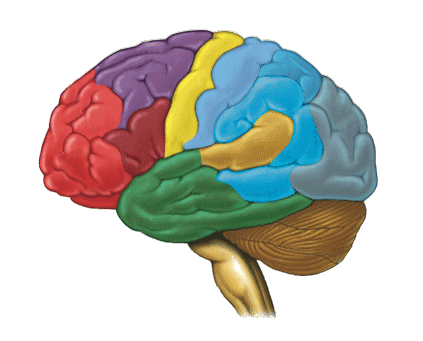
\includegraphics{phisio/mozg_2}};
		
		\node at (5,1.7) {Иерархия автоматов};
		\node[align=center] at (5,0) {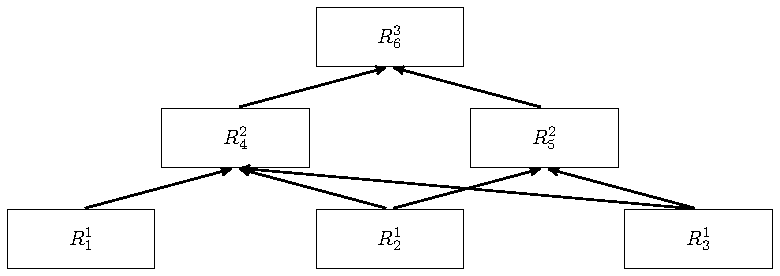
\includegraphics[width=0.4\textwidth]{rb_hierarchy}};
		
		\node at (10,1.7) {Психические функции};
		\node[align=center] at (10,-0.2) {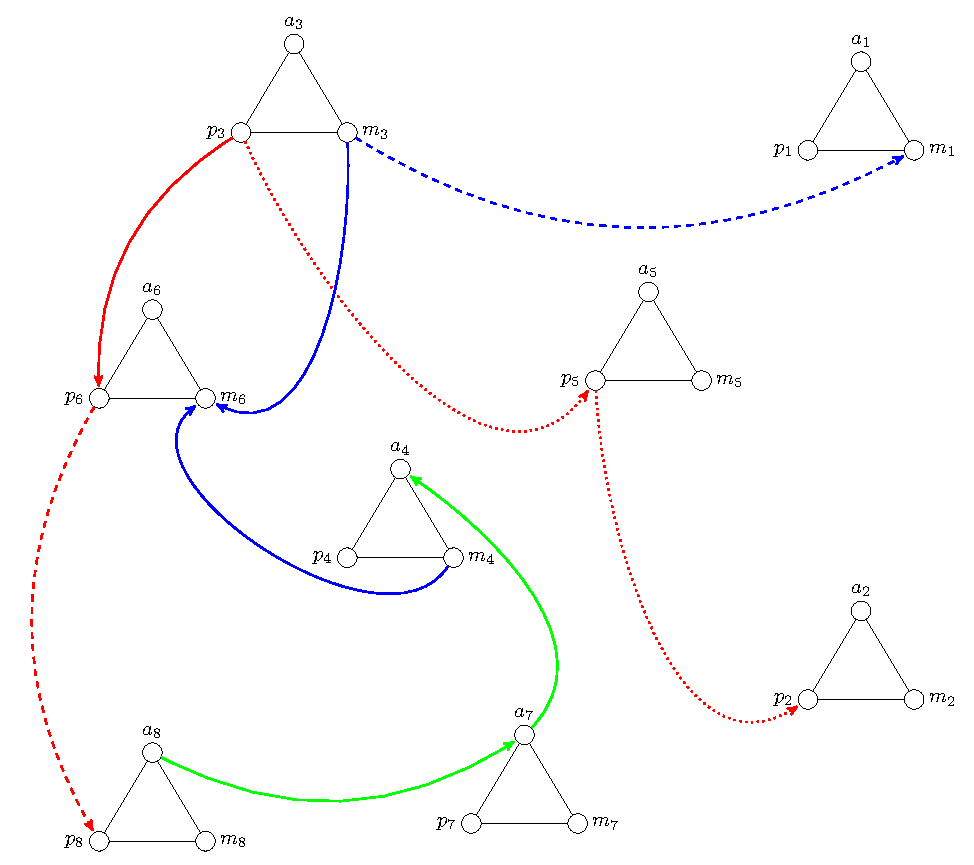
\includegraphics[width=0.3\textwidth]{signs/signs_net}};
		
		\node at (2.5,-2.3) {Внешняя среда};
		\draw[ultra thick] (1,-2.5) -- (1,-2) -- (4,-2) -- (4,-2.5);
		\scriptsize
		\draw[->,thick] (2,-2) edge[bend right] node[yshift=-15, left,align=center] {сенсорный\\вход} (1.4,-0.1);
		
		\draw[->,thick] (3,-2) -- (3.2,-0.8);
		\draw[->,thick] (3,-2) -- (5.0,-0.8);
		\draw[->,thick] (3,-2) -- node[yshift=-5, right, align=center] {входны\\автоматов} (7.0,-0.8);
		
		\draw[->, thick, color=red] (2.8,-0.6) edge[bend right] (1.1,0);
		\draw[->, thick, color=red] (3.9,0) edge[bend right] (-0.3,-0.2);
		\draw[->, thick, color=red] (4.7,0.7) edge[bend right] (-1.1,0.2);

		\draw[->] (5.1,0.8) edge[bend left] (9,0.9);
		\draw[->] (6.1,0.2) edge[bend left] (8.5,-0.1);		
	\end{tikzpicture}

\end{document}